A triangular array of squares has one square in the first row, two in the second, and in general, $k$ squares in the $k$th row for $1 \leq k \leq 11.$ With the exception of the bottom row, each square rests on two squares in the row immediately below (illustrated in given diagram). In each square of the eleventh row, a $0$ or a $1$ is placed. Numbers are then placed into the other squares, with the entry for each square being the sum of the entries in the two squares below it. For how many initial distributions of $0$'s and $1$'s in the bottom row is the number in the top square a multiple of $3$?
\begin{center}
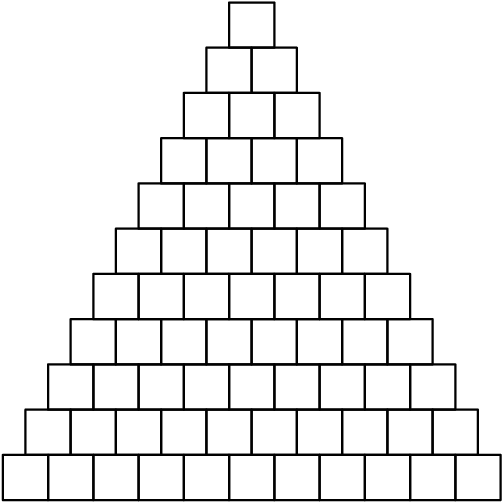
\includegraphics[width = 50.400000000000006mm]{img/fig0.png}
\end{center}